\documentclass{standalone}

\usepackage{tikz}
\usetikzlibrary{shapes}

\begin{document}
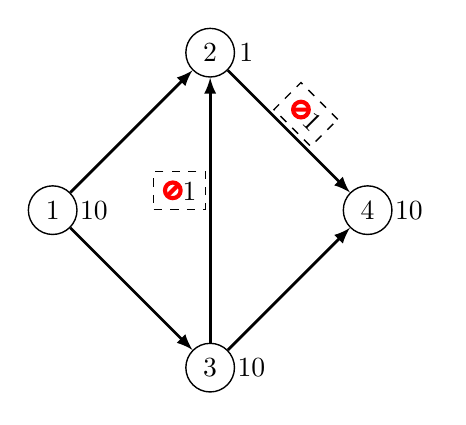
\begin{tikzpicture}
\tikzstyle{every path}=[-latex,line width=1pt]
\tikzstyle{every node}=[circle,draw,line width=0.5pt]
\tikzstyle{list}=[rectangle]

\begin{scope}
\node (1) [label={[xshift=-5pt]0: 10}] {1};
\node (2) at (2,2) [label={[xshift=-5pt]0: 1}] {2};
\node (3) at (2,-2) [label={[xshift=-5pt]0:10}] {3};
\node (4) at (4,0) [label={[xshift=-5pt]0:10}] {4};
\draw[-latex] (1)--(2);
\draw[-latex] (1)--(3);
\draw[-latex] (3)-- node[midway,rectangle,above,xshift=-11pt,dashed]
{\tikz{\tikzstyle{every path}=[-]\node[forbidden sign,draw,solid,red,line
width=1.5pt,scale=0.6] {};}1} (2);
\draw[-latex] (2)-- node[rectangle,midway,sloped,above,dashed,yshift=1.5pt]
{\tikz{\tikzstyle{every path}=[-]\node[forbidden sign,draw,solid,red,line
width=1.5pt,scale=0.6] {};}1} (4);
\draw[-latex] (3)--(4);
\end{scope}

\end{tikzpicture}
\end{document}

